\section{Handbook of Engineering Acoustics}

This book contains a chapter about the effects of sound on humans. First a small
overview of the perceptual processes and their associated perceptual quantities
is given. Table \ref{tab:stimsens} summarizes all the perceptual measures, along
with their dominant physical stimuli. It is interesting to note that all these
perceptual dimensions, except for density, were derived from the
``Munich school'' work of Zwicker and Fastl \cite{Fastl2007Psychoacoustics}.

\begin{table}
    \centering
    \tabulinesep = 4pt
    \begin{tabu}{ l l }
        \tabucline[1pt]{-}
        Dominant stimuli & Cognitive parameters \\\tabucline[1pt]{-}
        Sound pressure level (dB) & Loudness (sone) \\\cline{2-2}
        & Loudness level (phon) \\\hline
        Frequency (Hz) & Critical band rate (Bark) \\\cline{2-2}
        & Ratio pitch (mel) \\\hline
        Degree of modulation (\%) & Roughness (asper)\\\cline{1-1}
        Modulation frequency (Hz) & \\\hline
        Frequency (Hz) & Sharpness (acum) \\\hline
        Degree of modulation (\%) & Fluctuation strength (vacil) \\\cline{1-1}
        Modulation frequency (Hz) & \\\hline
        Spectral components (Pa) & Pitch strength \\\cline{2-2}
        & Tonality (tu) \\\hline
        Impulse duration (s) & Subjective duration of impetus (IU) \\\hline
        Sound pressure level (dB) & Density (dasy) \\
        Frequency (Hz) & \\\tabucline[1pt]{-}
    \end{tabu}
    \caption{Stimuli and sensations \cite[pp. 72]{Mueller2012Handbook}}
    \label{tab:stimsens}
\end{table}

It is important to note that the human auditory system can generate these
perceptual sensations independently of each other, although to understand the
general ``pleasantness'' of a sound a bigger context needs to be taked into
account. For instance the emotions of the listeners can have an important
effect on the cognitive construal of a given sound.

\subsection{Fluctuation Strength}

Fluctuation strength corresponds to the sensation that arises when a sound
presents a slow amplitude envelope (a modulation signal with less than 20 Hz).
Fluctuation strength is closely related to roughness, the difference between the
two being the frequency of the amplitude envelope. As a reference, the unit of 1
vacil is defined as a 1 kHz tone sound having a SPL of 60 dB, with an
amplitude-modulated envelope of 4 Hz with a modulation index of 1. The maximum
of this quantity seems to occur around 4 Hz regardless of the modulation
technique used (amplitude or frequency modulation), as seen from Figure
\ref{fig:flucstrenvmodfreq}.

\begin{figure}
    \centering
    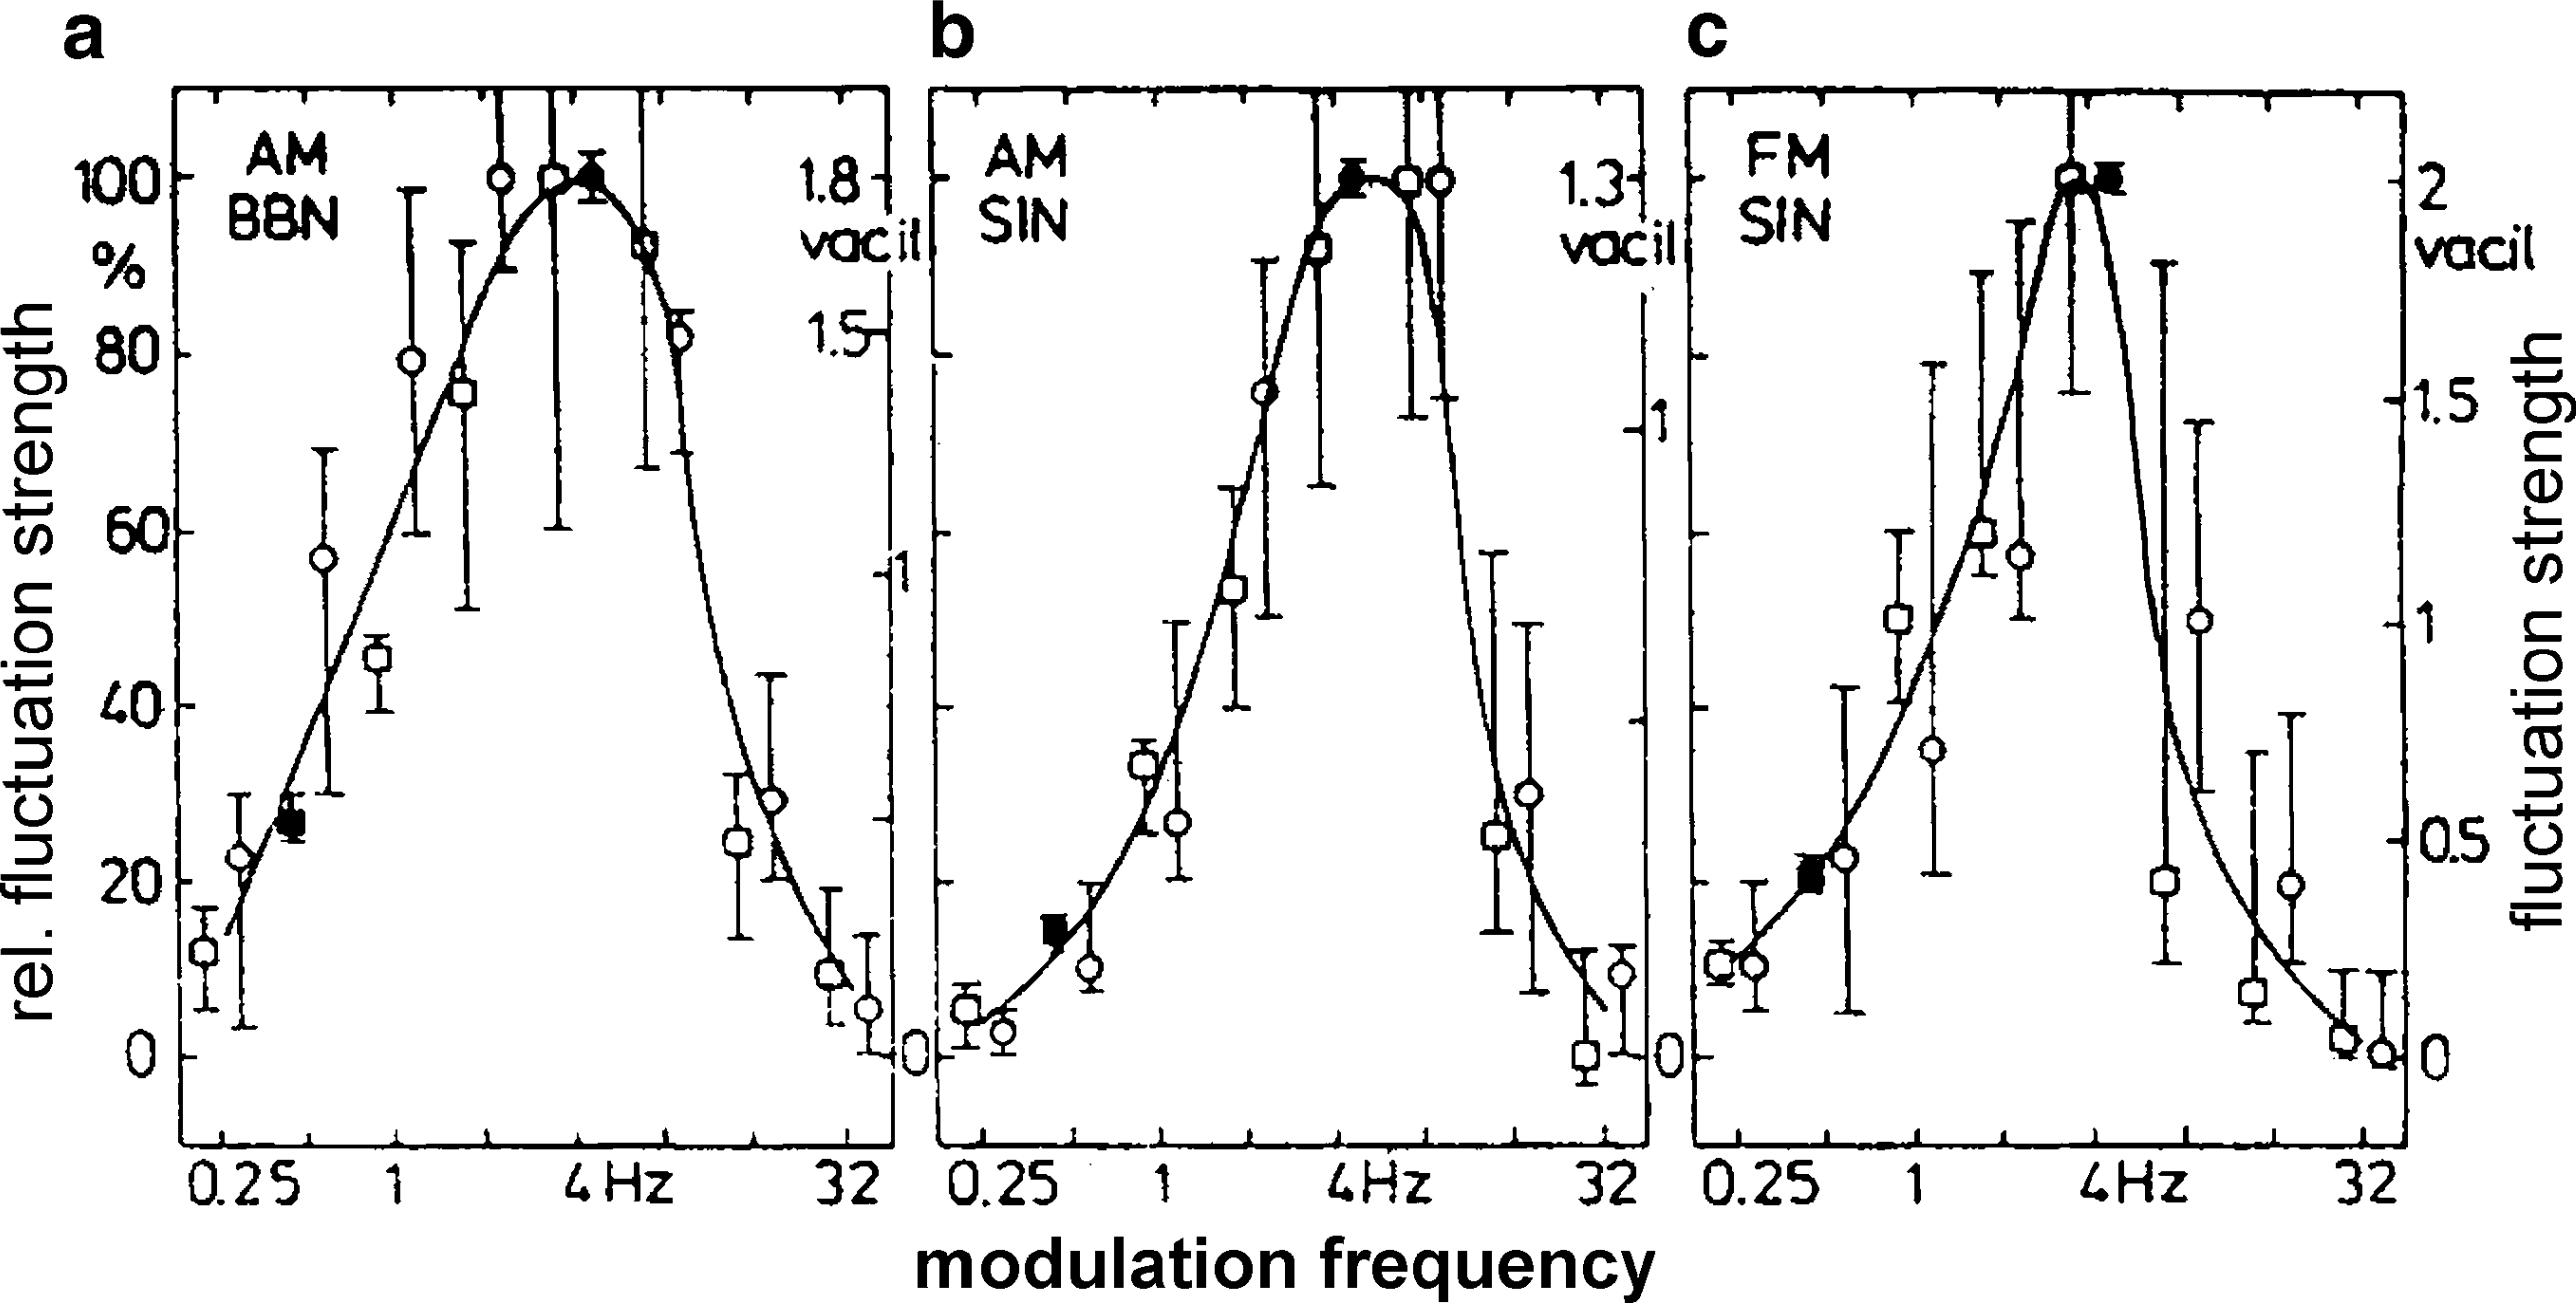
\includegraphics[height=5cm]
        {Mueller2012Handbook-FluctuationStrengthVsModulationFrequency}
    \caption{Fluctuation of strength vs. modulation frequency for
        amplitude-modulated broad-band noise (a), an amplitude-moduled tone (b)
        and a frequency-modulated tone (c) \cite[pp. 75]{Mueller2012Handbook}}
    \label{fig:flucstrenvmodfreq}
\end{figure}

Fluctuation strength can have a significant effect on the pleasantness of a
a sound, and a particularly clear example of this are alarms, which must have a
sharp and distinctive sound.

The effect of fluctuation strength can be seen as a temporary masking pattern on
an original signal, in which the modulation depth is of utmost importance. This
is also the case for roughness, which resembles fluctuation strength in this
regards.
